\begin{itemize}
\item Gamification is not Playful design or gameful design:
\end{itemize}

Playful design is using game-based aesthetics or limited usability
based on game elements in non-game contexts with the purpose of
drawing the user's attention \cite{Ferri2017}. These elements are used to amuse
users and cause an emotional response. One successful example is
Twitter’s page knows as “Fail Whale” (Figure~\ref{fig:failwhale}). Whenever
there is an overload on the servers, instead of a boring page with
some standard error message, users are presented with a drawing of
a dozen birds, twitters, trying to lift a whale \cite{kalbach2016mapping}.

% Playful design or gameful design
\begin{figure}[h!]
\caption{The (now retired) “Fail Whale” was used to illustrate Twitter's service outage.}
\centering
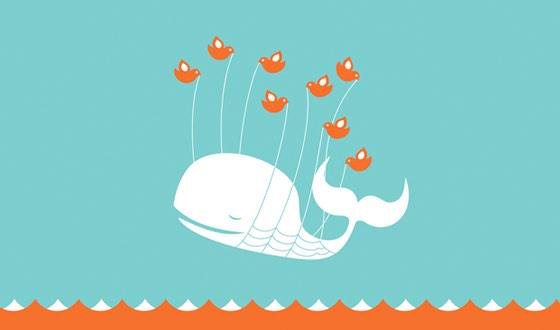
\includegraphics[width=0.4\textwidth]{failwhale}
\label{fig:failwhale}
\end{figure}

\begin{itemize}
\item Gamification is not Serious games:
\end{itemize}

Serious games are games designed for non-recreational
environments, however with learning and game objectives in focus \cite{Blanchard2011}. The term
“serious” is employed because these games can focus on areas as
diverse as economics, education, health, industry, military,
engineering, and politics. In environments created by applying
serious game concepts, it is possible to simulate real-world
situations without incurring in eventual costs and risks. The main
goal of this sort of training-environment is to convey information
to the user. The Virtual Incident Management Training System
(Figure~\ref{fig:serious_games}) is a multiplayer training environment designed for
training professionals that need to act swiftly in case of accident on
highways, such as paramedics and policemen \cite{catt_lab2017}.

% Serious game
\begin{figure}[h!]
\caption{The Virtual Incident Management Training System initial screen. Source: \cite{catt_lab2017}}
\centering
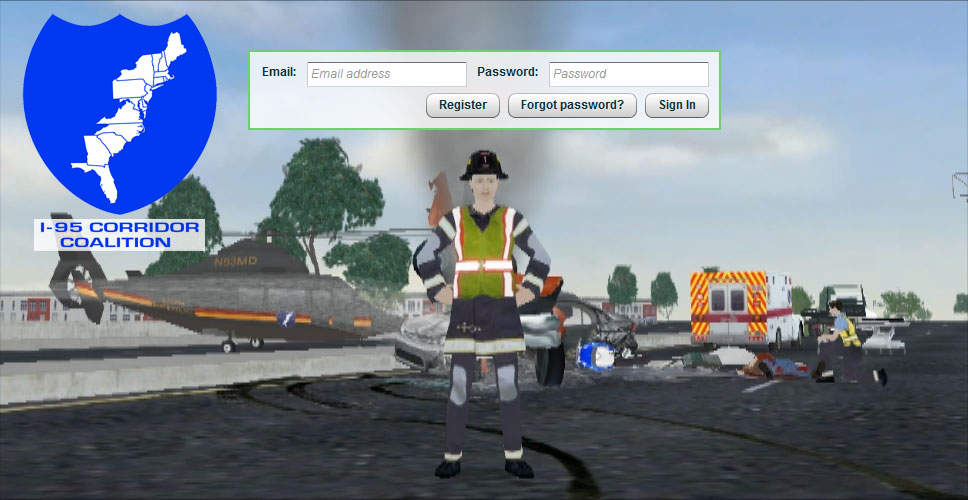
\includegraphics[width=0.5\textwidth]{serious_games}
\label{fig:serious_games}
\end{figure}

\begin{itemize}
\item Gamification is not video games or digital games:
\end{itemize}

Video Games or Digital Games are systems in which users are
engaged in resolving abstract conflicts and challenges, under
predetermined rules \cite{fullerton2008}. In this scenario the game continuously
offers interactivity and feedback to the user, which often result in
an emotional reaction. Figure 1-d shows a screenshot of the game
New Super Mario Bros.Wii\copyright whose main character, Mario, is
considered one of the most iconic video game characters.

% Video games or Digital games
\begin{figure}[h!]
\caption{New Super Mario Bros.wii a game developed and publishid by Nintendo}
\centering
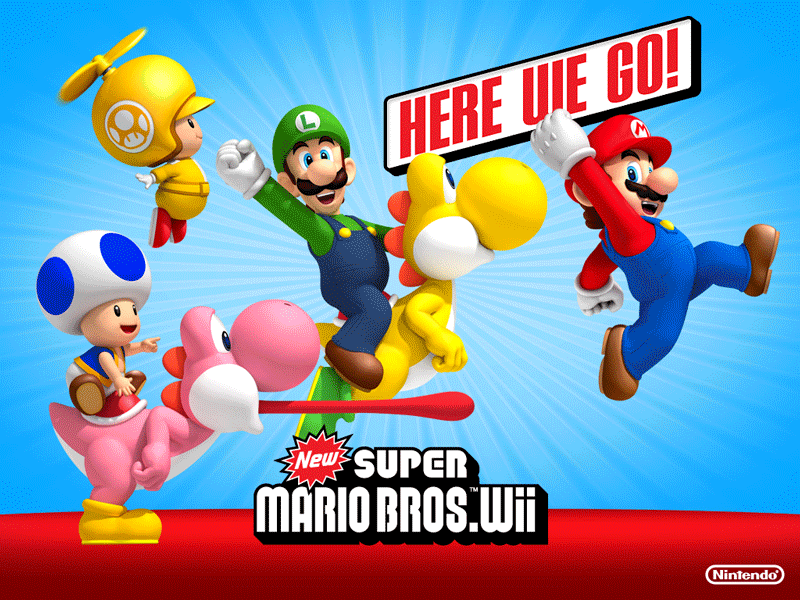
\includegraphics[width=0.4\textwidth]{super_mariowii}
\label{fig:super_mariowii}
\end{figure}
